\section{Experiment}
The experiment took place over two weekends in central Aalborg, Denmark. Participants used an iPad 2 3G + WiFi as the platform. To investigate the effects of riddle solving as the navigation method in a location-based game, we conducted a comparative study between navigating by riddle solving and navigating by a 2D map with GPS. 

\subsubsection{Hypothesis}
We hypothesized that \textit{riddle solving as a navigational method is more enjoyable than maps.} We came up with the following null hypothesis and its alternative hypothesis. 

\textbf{H0:} Riddle solving as navigational method is equally or less enjoyable than maps. 

\hspace{10 mm} \textit{H0: $\mu$EnjoyabilityRiddle $\leq$ $\mu$EnjoyabilityMap}

\textbf{H1:} Riddle solving as navigational method is more enjoyable than maps.

\hspace{10 mm} \textit{H1: $\mu$EnjoyabilityRiddle $>$ $\mu$EnjoyabilityMap}

\subsubsection{Participants}
We recruited 10 families of 2-6 persons through posters and flyers at schools. 
As the narrative of the game was targeted children, it was a requirement that the families had at least one child in the age range 9-11 years old. 17 children participated with ages ranging between 7 and 13 (mean = 10.1, SD = 1.6), 9 females and 8 males. 14 adults participated with ages ranging between 36 and 62 (mean = 42.3, SD = 6.4), 4 females and 10 males.  All participants lived in the city Aalborg or nearby, and were familiar with the city (4 went to the city daily, 5 went to the city weekly, 18 went to the city monthly, 4 went to the city yearly). All participants were familiar using tablet or mobile devices (23 used it daily, 6 used it weekly, 1 used it monthly, 1 used it yearly).

\subsubsection{Materials and Procedure}
The experiment was designed as a within-subjects design with two conditions. (1) A navigational method, where the participants navigated by solving riddles (R) and (2) A navigational method in which the participants used a digital map (M).

These two conditions were counterbalanced with the purpose of reducing the environmental effects met on the route on the results. Participants would either begin with map or riddles, and would end with the navigational method different from the one met in the beginning. 

Three street arts, A, B and C, were a part of the experience. The distance from A to B was 0,9 km and the distance from B to C was 0,9 km. Each condition also had approximately same amount of turns, respectively 8 and 7 turns. Each session lasted between 31 minutes and 40 seconds to 50 minutes and 55 seconds. One facilitator and  an assisting facilitator were present during the whole session. The facilitator instructed the participants in using the application before the experiment took place, and further helped during the game if any difficulties arised (e.g. participants got lost). For each session, one of the parents was instructed to wear a GoPro with a harness for recording video, while one of the children carried a bluetooth microphone for recording audio. All parents signed consent forms and filled out demographic questionnaires prior to the experience. We gave the child in the age range 9-11 years old the iPad, but they were not forced to handle it the whole session. 

LBGs have previously been evaluated using both qualitative and quantitative methods including observational studies, questionnaires and interviews. Morrison et. al. used Flow \cite{GameFlow} , Instrinsic Movation (IMI) \cite{whatwhy} and Presence - MEC-SPQ \cite{Presence} questionnaires and successfully evaluated effects such as enjoyability, intrinsic motivation and awareness of surroundings by triangulating with video recordings, logs, field notes and transcriptions of interview data. We used the same approach, based on the success of Morrison et al. investigating similar criteria as our study. 

The questionnaires in this study contains questions from the Short Flow State Scale Questionnaire (S-FSS 2), which measures the degree to which flow dimensions characterize the
complete experience\cite{flowfss}. The questionnaire also contains questions from IMI (measures enjoyability, tension, effort and perceived competence) and MEC-SPQ (measures spatial presence, allocated attention and suspension of disbelief). Only adults received this questionnaire due to the level of complexity, while children received a simplified questionnaire measuring enjoyability using IMI. Both questionnaires were measured on a likert scale (5-scale), going from 1 (strongly disagree) to 5 (strongly agree). The parents were instructed to help the children to fill out the questionnaire in terms of them having difficulties. Logging, field notes, interview and video data was used for supporting the analysis of questionnaires. Findings from the analysis is presented in the following section. 
 
\section{Results}

\subsection{Observations}
During the experiment, the facilitator walked behind the families and took general notes on the interaction of both conditions. It must be noted that the following observations have not been coded, e.g. through video analysis, but are based on general tendencies.

The biggest differences between the two conditions could be seen in regards to the participants' social behaviour. In general, there was more communication between participants during riddle navigation than during map and the topics were different. During riddles, participants primarily talked about the environment and collaborated to solve the riddles, while during map navigation participants tended to talk about things outside of the game, e.g. one child started talking about his soccer practice. However, this mostly tended to happen on long paths without intersections, as these areas require less attention from users during map navigation. From this, it seems that riddles in general require more attention than maps (See Figure \ref{Communication}). 

\begin{figure}[hbtp]
\centering
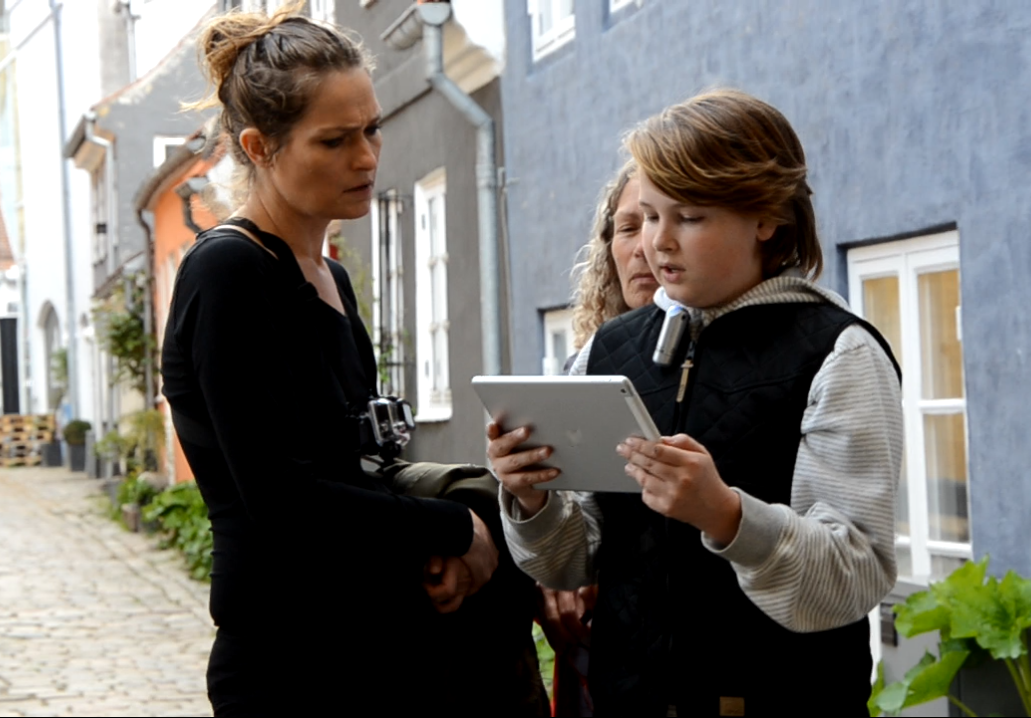
\includegraphics[scale=0.15]{Pics/exp1.png}
\caption{All participants attending to the iPad, trying to solve the riddle}
\label{Communication}
\end{figure}

For both conditions, collaboration was mostly seen between the child using the iPad and a parent. Here, the parent would act as an assistant to the child and take over the iPad if the child gave up (See Figure \ref{Communication2}). If there were multiple children, the children not holding the iPad would often have a hard time participating in the navigation and would just follow the group. This indicates that the design does not fully encourage collaboration between multiple players, and it is possible that the collaboration between child and parent naturally arises from the fact that parents are used to assisting their children. During this collaboration however, it was clear that if the riddles were too difficult for the children, but the parents knew the answer, the parents would give their children hints in order for them to solve the riddle. From this, it could be seen that harder riddles encouraged more communication and collaboration.

\begin{figure}[hbtp]
\centering
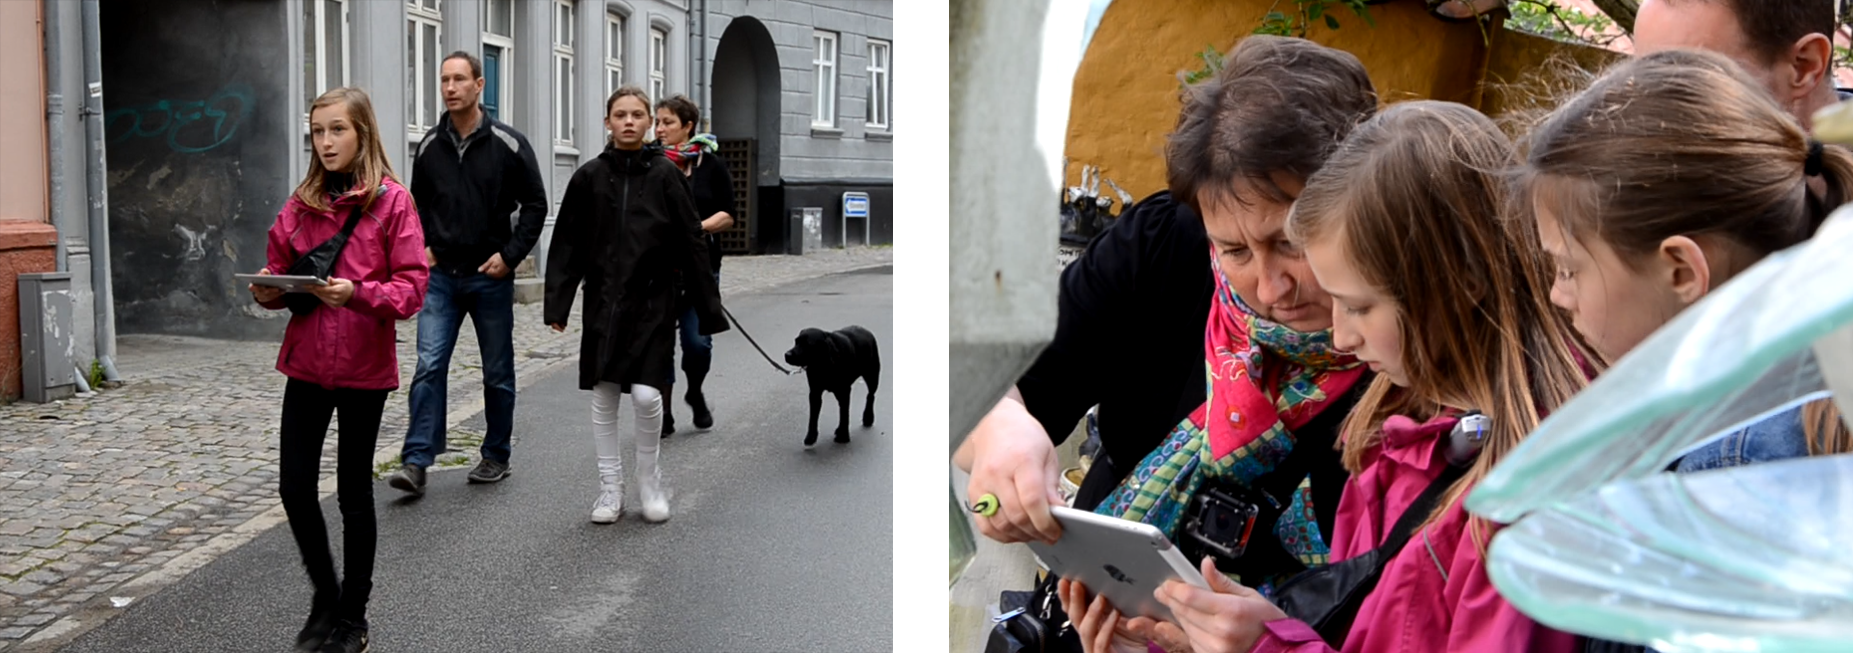
\includegraphics[scale=0.13]{Pics/exp2.png}
\caption{Child in charge of the iPad (left) and parent assisting the child (right)}
\label{Communication2}
\end{figure}

Regarding the riddle system, it was clear that a better explanation of the system to the participants is needed. Often participants would answer the riddles without going to the position of the previous landmark first, which caused frustration since participants would not be able to find the landmarks used in the riddles. Especially families that used riddle navigation for the second part of the route, had a hard time understanding the system. This indicates that the tutorial built into the system did not provide clear enough instructions. Furthermore, the riddle system is shortly explained by the facilitator in the beginning of the experiment, and this information might have been forgotten as participants reached the second part of the route. 

%This problem could be solved by simply having the facilitator explain the riddle system as the participants start the first riddle

When navigating using the map, the participants' current position on the map was often slow at updating due to the lack of a proper GPS signal. This caused participants to walk down wrong paths, and it could take several minutes for the signal to be re-established, causing confusion in the participants. As a result some participants ended up reaching the destination by taking completely different paths, and in one case, it was necessary for the facilitator to guide the participants.

Finally, it was observed that people in general looked around and paid more attention to the environment when solving riddles than when using a map. During map navigation, the participant holding the iPad primarily looked down on the iPad, and it was mostly at intersections that participants looked around in the environment. It was also observed that especially when the GPS signal was weak during map navigation that participants looked down on the iPad. 	
%Children could easily get distracted by things in the environment for both conditions (e.g. dogs)	
%"Nu får vi styr på Aalborg"
\subsection{Questionnaires}
We used the Wilcoxon Signed-Rank test, based on the nature of ordinal values and because the sample had been exposed to two conditions (riddle solving and map).

All participants found the system using riddles significantly more intrinsically motivating (IMI) than maps (See Table \ref{my-label1}). Assessing IMI, we found that enjoyability and effort scores were significantly higher for riddles compared to maps. Riddles also received a significantly higher score than maps concerning total flow. No significant difference was found for presence, but riddles was still favoured in terms of its score. 

\begin{table}[h]
\caption{Questionnaire items showing significant differences between riddle-based navigation and map navigation}
\label{my-label1}
\begin{tabular}{lll}
\hline
\multicolumn{1}{|l|}{\textbf{\begin{tabular}[c]{@{}l@{}}Item and Wilcoxon\\ Signed-Rank Test\end{tabular}}} & \multicolumn{1}{l|}{\textbf{\begin{tabular}[c]{@{}l@{}}System\\ with higher\\ mean\end{tabular}}} & \multicolumn{1}{l|}{\textbf{\begin{tabular}[c]{@{}l@{}}System\\ with lower\\ mean\end{tabular}}} \\ \hline
\multicolumn{3}{|l|}{\cellcolor[HTML]{EFEFEF}\textit{Item related IMI for \textbf{all participants}}}                                                                                                                                                                                                                                    \\ \hline
\multicolumn{1}{|l|}{IMI - total(**)}                                                                       & \multicolumn{1}{l|}{\begin{tabular}[c]{@{}l@{}}Riddle\\ Mean=4.31\end{tabular}}                  & \multicolumn{1}{l|}{\begin{tabular}[c]{@{}l@{}}Map\\ Mean=3.64\end{tabular}}                    \\ \hline
\multicolumn{1}{|l|}{IMI - Enjoyment(**)}                                                                   & \multicolumn{1}{l|}{\begin{tabular}[c]{@{}l@{}}Riddle\\ Mean=4.49\end{tabular}}                  & \multicolumn{1}{l|}{\begin{tabular}[c]{@{}l@{}}Map\\ Mean=3.46\end{tabular}}                    \\ \hline
\multicolumn{1}{|l|}{IMI - Pressure(-)}                                                                     & \multicolumn{1}{l|}{\begin{tabular}[c]{@{}l@{}}Map\\ Mean=2.11\end{tabular}}                     & \multicolumn{1}{l|}{\begin{tabular}[c]{@{}l@{}}Riddle\\ Mean=1.78\end{tabular}}                 \\ \hline
\multicolumn{1}{|l|}{IMI - Effort(*)}                                                                       & \multicolumn{1}{l|}{\begin{tabular}[c]{@{}l@{}}Riddle\\ Mean=4.30\end{tabular}}                  & \multicolumn{1}{l|}{\begin{tabular}[c]{@{}l@{}}Map\\ Mean=3.68\end{tabular}}                    \\ \hline
\multicolumn{1}{|l|}{IMI - Perceived Competence(-)}                                                         & \multicolumn{1}{l|}{\begin{tabular}[c]{@{}l@{}}Riddle\\ Mean=4.13\end{tabular}}                  & \multicolumn{1}{l|}{\begin{tabular}[c]{@{}l@{}}Map\\ Mean=3.68\end{tabular}}                    \\ \hline
\multicolumn{3}{|l|}{\cellcolor[HTML]{EFEFEF}\textit{Item related Flow only for \textbf{adults}}}                                                                                                                                                                                                                                             \\ \hline
\multicolumn{1}{|l|}{Flow - total(*)}                                                                       & \multicolumn{1}{l|}{\begin{tabular}[c]{@{}l@{}}Riddle\\ Mean=3.85\end{tabular}}                  & \multicolumn{1}{l|}{\begin{tabular}[c]{@{}l@{}}Map\\ Mean=3.60\end{tabular}}                    \\ \hline
\multicolumn{3}{|l|}{\cellcolor[HTML]{EFEFEF}\textit{Item related Presence only for \textbf{adults}}}                                                                                                                                                                                                                                         \\ \hline
\multicolumn{1}{|l|}{Presence - total(-)}                                                                   & \multicolumn{1}{l|}{\begin{tabular}[c]{@{}l@{}}Riddle\\ Mean=3.07\end{tabular}}                  & \multicolumn{1}{l|}{\begin{tabular}[c]{@{}l@{}}Map\\ Mean=2.95\end{tabular}}                    \\ \hline
\multicolumn{3}{l}{\begin{tabular}[c]{@{}l@{}}Note: (-) = p\textgreater.05 and (*) = p\textless.05 and (**) = p\textless.01\\ IMI, Flow and Presence 1-5 scale\end{tabular}}                                                                                                                                      
\end{tabular}
\end{table}

We found significant differences when assessing individual questions from the questionnaire (See Table \ref{my-label}). All participants especially found the riddle system significantly more fun and less boring compared to the map version. As previously mentioned, we observed that riddles were able to include multiple family members, which  accommodate the fact that all participants had an enjoyable experience. 

Adults found the riddles significantly more rewarding and had the feeling of time moving faster compared to the map version. These two questions specifically assesses the dimension on having an autotellic experience and the sense of time transformation. As flow involves nine dimensions, these two were the only dimensions to reveal a significant difference. Other dimensions of flow favoured riddles, or were closely tied with maps (0.05 score difference between riddles and maps), except for a flow question revolving on clear goals. Our questionnaire revealed that test participants found the map system had more clear goals (R = 3.31, M = 3.83, p =.174). As the result is not significant, it is however observed that the map did not require much training, and henceforth more intuitive than what we observed with the riddle system. However, participants still favoured the riddle system despite these difficulties. 

Children thought they were significantly better at navigating with riddles than maps. In line with that, children also considered maps more challenging, which could provide an explanation on the matter, but this outcome was not significant (R = 2.82, M = 3.33, p = .177).
 
We performed a multiple ordinal regression analysis on the questions from Table \ref{my-label} in order to investigate, whether age, gender, condition order or group size served as predictors for the results. In all cases, the results stayed significant, but the condition order had a significant impact on several of the questions concerning IMI. Due to the condition order, the selection of riddles was different for each condition, as well as the route described on the map. Participants met different landmarks on the route based on the condition order, which eventually provided a different experience between conditions. 

\begin{table}[h]
\caption{Questionnaire items showing significant differences between riddle navigation and map navigation}
\label{my-label}
\begin{tabular}{|l|l|l|}
\hline 
\textbf{\begin{tabular}[c]{@{}l@{}} Item and Wilcoxon \\ Signed-Rank Test\end{tabular}} & \textbf{\begin{tabular}[c]{@{}l@{}}System\\ with higher \\ mean\end{tabular}} & \textbf{\begin{tabular}[c]{@{}l@{}}System \\ with lower \\ mean\end{tabular}} \\ \hline
\rowcolor[HTML]{EFEFEF} 
\hline
\multicolumn{3}{|l|}{\cellcolor[HTML]{EFEFEF}\textit{Items related\textbf{ all participants}}} \\ \hline
\begin{tabular}[c]{@{}l@{}}IMI: I thought navigating\\ was fun (**)\end{tabular} & \begin{tabular}[c]{@{}l@{}}Riddle\\ Mean=4.48\end{tabular} & \begin{tabular}[c]{@{}l@{}}Map\\ Mean=3.42\end{tabular} \\ \hline
\begin{tabular}[c]{@{}l@{}}IMI: I thought navigating\\  was boring (R) (**)\end{tabular} & \begin{tabular}[c]{@{}l@{}}Map\\ Mean=2.14\end{tabular} & \begin{tabular}[c]{@{}l@{}}Riddle\\ Mean=1.41\end{tabular} \\ \hline
\begin{tabular}[c]{@{}l@{}}Flow: My attention was\\ focused on navigating (*)\end{tabular} & \begin{tabular}[c]{@{}l@{}}Riddle\\ Mean=4.16\end{tabular} & \begin{tabular}[c]{@{}l@{}}Map\\ Mean=3.66\end{tabular} \\ \hline
\rowcolor[HTML]{EFEFEF} 
\multicolumn{3}{|l|}{\cellcolor[HTML]{EFEFEF}\textit{Items related only \textbf{adults}}} \\ \hline
\begin{tabular}[c]{@{}l@{}}Flow: I found the experience\\  highly rewarding (*)\end{tabular} & \begin{tabular}[c]{@{}l@{}}Riddle\\ Mean=3.93\end{tabular} & \begin{tabular}[c]{@{}l@{}}Map\\ Mean=3.15\end{tabular} \\ \hline
\begin{tabular}[c]{@{}l@{}}IMI: I enjoyed\\  navigating a lot (*)\end{tabular} & \begin{tabular}[c]{@{}l@{}}Riddle\\ Mean=4.29\end{tabular} & \begin{tabular}[c]{@{}l@{}}Map\\ Mean=3.46\end{tabular} \\ \hline
\begin{tabular}[c]{@{}l@{}}Flow: It felt like time\\  went by quickly (*)\end{tabular} & 
\begin{tabular}[c]{@{}l@{}}Riddle\\ Mean=4.54\end{tabular} & \begin{tabular}[c]{@{}l@{}}Map\\ Mean=3.69\end{tabular} \\ \hline
\rowcolor[HTML]{EFEFEF} 
\multicolumn{3}{|l|}{\cellcolor[HTML]{EFEFEF}\textit{Items related only \textbf{children}}} \\ \hline
\begin{tabular}[c]{@{}l@{}}IMI: I thought I was pretty\\  good at navigating (*)\end{tabular} & 
\begin{tabular}[c]{@{}l@{}}Riddle\\ Mean=4.41\end{tabular} & \begin{tabular}[c]{@{}l@{}}Map\\ Mean=3.73\end{tabular} \\ \hline
\multicolumn{3}{l}{\begin{tabular}[c]{@{}l@{}}Note: (*) = p\textless.05 and (**) = p\textless.01. \\ IMI and Flow 1-5 scale\end{tabular}}
\end{tabular}
\end{table}
 
From these findings, we can reject our null hypothesis, stating that riddle solving as a navigational method is more enjoyable than maps.

\subsection{Interviews}
Despite results from questionnaires being statistically significant, showing that riddle solving is a more enjoyable navigational method than maps, findings from interview data allowed for deeper analysis into the effects of this method. From interview data, we found that 5 out of 22 children expressed preference towards using maps. One parent mentioned she also preferred map, saying \textit{"It is just always fun to follow a map"}. This parent explained that they were unsure about what to do during the riddle-based navigation and could not remember what they had been told during the instructions. 

Another parent mentioned that map was easy and did not make one aware of the surroundings, because the focus was on walking. In general, we found different opinions on whether the different navigational methods made people aware of the surroundings. One parent clearly stated the the children were not interested in the map at all. In line with several other test participants this parent expressed that it was fun to notice things in the environment they usually do not notice when walking by, making it an optimal method for tourists. Opposed to that opinion, another parent expressed that she focused more on navigating than noticing things in the environment. With riddles, one parent felt that the attention was on the next location to go to, while the map made the participant more aware of the city, because there was more time to look around in the surroundings. 

When asked if they would use riddles as navigational method, if they were to use it in another city, all test participants agreed and answered yes. Some thought it would be a more fun way of learning the city, finding the way and that it would make it possible to see the city in a different way. However, interview data also clearly revealed that several participants would have enjoyed it more, if the riddles were about more interesting landmarks that gave the possibility to learn more e.g. about the city. Preferably this should be done with the children in mind and a few parents proposed a system that can be adjusted depending on, whether they had any children and adjusted content according to the children’s age. Riddles as navigational method was described as \textit{"fun if you have time for it"} by one parent. 

The most used word to describe riddle-based navigation was "fun" (11 of 29 words). This reflected the results from the questionnaires. Other words included exciting, challenging, different, educational and inspiring. Some participants thought it was fun to answer the questions after the riddles, particularly one child mentioned that it was fun to be able to answer correctly to questions. Results from the log further showed a high tendencies of correct answers to control questions (in average 96,9 \% of the control questions across all sessions were answered correctly), indicating that the feedback system had an impact on the enjoyability of the game. One parent mentioned that the fun part in the riddle-based navigation was to help each other and agree on what they have seen in the environment. Several parents had a similar opinion and stated that they enjoyed collaborating and discussing the answers with the other family members. One parent said it was fun with riddles, 

\begin{quote}
    "(...) because there was something to discuss. Of course you can also discuss what way to go with the map, but that just gave a different experience."
\end{quote}

In terms of group dynamics, it was mentioned that primarily the one with the device was in control (See Figure \ref{Communication}), making it a less collaborative experience. One parent mentioned that they collaborated more, when navigating using riddles and not as much with the map. In order to make it more collaborative, one of the participants suggested making the riddles more difficult, encouraging the participants to help each other. This statement supports the experience of another parent, who mentioned that they only collaborated when there was any doubt, otherwise they just followed the child, who was mostly in charge of the device. 

The interview data revealed a tendency to let the child control the device, which was described as following by one parent,  

\begin{quote}
    "Then one finds out about something and the other finds out about something else. I 
felt I gave much of the control to Mikki (the child), because I wanted him to think it 
was fun."
\end{quote}
 
In one family, the parent stated that it was much more fun for them both, when the child had the device, because the child was better at using the map and tablets in general.